\documentclass[10pt,twocolumn,letterpaper,UTF8]{article}

\usepackage{cvpr}
\usepackage{times}
\usepackage{epsfig}
\usepackage{graphicx}
\usepackage{amsmath}
\usepackage{amssymb}
\usepackage{mathtools}

\usepackage{color}
\usepackage{subfigure}
\usepackage{booktabs}
\usepackage{amsthm}
\usepackage{ctex}
\usepackage{abstract}

% Include other packages here, before hyperref.

\usepackage[breaklinks=true,bookmarks=false,hidelinks=true]{hyperref}
\usepackage[hyphenbreaks]{breakurl}

%%Fix for tables. Source: http://www.tex.ac.uk/FAQ-floats.html
\renewcommand{\topfraction}{.85}
\renewcommand{\bottomfraction}{.7}
\renewcommand{\textfraction}{.15}
\renewcommand{\floatpagefraction}{.66}
\renewcommand{\dbltopfraction}{.66}
\renewcommand{\dblfloatpagefraction}{.66}

% https://tex.stackexchange.com/questions/12703/how-to-create-fixed-width-table-columns-with-text-raggedright-centered-raggedlef#12712
\usepackage{array}
\newcolumntype{L}[1]{>{\raggedright\let\newline\\\arraybackslash\hspace{0pt}}m{#1}}
\newcolumntype{C}[1]{>{\centering\let\newline\\\arraybackslash\hspace{0pt}}m{#1}}
\newcolumntype{R}[1]{>{\raggedleft\let\newline\\\arraybackslash\hspace{0pt}}m{#1}}

\newcommand*{\thead}[1]{%
\multicolumn{1}{c}{\bfseries\begin{tabular}{@{}c@{}}#1\end{tabular}}}

\newcommand{\norm}[1]{\left\lVert#1\right\rVert}
\newcommand{\rpm}{\raisebox{.2ex}{$\scriptstyle\pm$}}

%%Convenience command for et al
%\newcommand{\etal}{et al.}

\newcommand{\specialcellbold}[2][c]{%
  \bfseries
  \begin{tabular}[#1]{@{}l@{}}#2\end{tabular}%
}

\cvprfinalcopy % *** Uncomment this line for the final submission

\def\httilde{\mbox{\tt\raisebox{-.5ex}{\symbol{126}}}}

% Pages are numbered in submission mode, and unnumbered in camera-ready
\ifcvprfinal\pagestyle{empty}\fi

\newtheorem*{claim}{Claim}

\begin{document}
% \renewcommand\thelinenumber{\color[rgb]{0.2,0.5,0.8}\normalfont\sffamily\scriptsize\arabic{linenumber}\color[rgb]{0,0,0}}
% \renewcommand\makeLineNumber {\hss\thelinenumber\ \hspace{6mm} \rlap{\hskip\textwidth\ \hspace{6.5mm}\thelinenumber}}
% \linenumbers

%\mainmatter

\title{定位没有边界框的目标}

\author{Javier Ribera, David G\"{u}era, Yuhao Chen, Edward J. Delp\\
    {视频与图像处理实验室 (VIPER), 普渡大学} \\
}

\maketitle
\ifcvprfinal\thispagestyle{empty}\fi


\begin{abstract}
    最近卷积神经网络研究进展(CNN)在图像中的目标定位方面取得了显著的效果。
    在这些网络中,训练过程通常需要提供边界框或者预期的目标的最大数量。
    在这篇论文中,我们解决了预估目标位置的任务并且没有使用标注的边界框,
    其中这些边界框通常需要手工绘制并且消耗时间去进行标注。
    我们提出了一个损失函数,可在任何全卷积网络(FCN)使用来预估对象位置。
    这个损失函数是两个无序点集之间的平均Hausdorff距离的改进。
    提出的方法没有边界框、候选区域或者滑动窗口的概念。
    我们使用三个数据集来评估我们的方法,这些数据集旨在定位人的头部、瞳孔中心和植物中心。
    我们的性能优于最先进的通用物体探测器和针对瞳孔跟踪进行微调的方法。
\end{abstract}

\section{介绍}

定位物体在图像中的位置在计算机视觉中是一件非常重要的任务。
在目标检测中一种普遍的方法是获取感兴趣对象周围的边界框。
在本文中,我们对获取边界框不敢兴趣。
相反,我们将目标检测任务定义为获取对应于每个对象位置的单个二维坐标。
目标的位置可以是我们感兴趣的任何关键点,比如它的中心。
图片~\ref{fig:collage} 展示了一个在图像中定位目标的例子。
与其它关键点检测问题不同,我们事先不知道在图像中关键点的数目。
为了使这个方法尽可能的通用,我们不假定点之间存在任何物理约束,这与姿态估计等情况不同。
这种对目标检测的定义更适合于对象非常小或者基本上重叠的应用(比如图片1中重叠的植物)。
在这些情况下,数据集可能不会提供边界框或者它们不可能得到真实的边界框(groundtruth)。

边界框的标注冗长、耗时且昂贵~\cite{Papadopoulos2015}。
例如,在Amazon的Mechanical Turk使用专门为边界框开发的高效标注技术进行众包~\cite{su2012},标注ImageNet~\cite{imagenet}中的每一个边界框需要42秒。
在~\cite{bell2015}中,Bell等人介绍了一个用于材料分类和分割的数据集。
通过在此数据集中收集单击位置的标签,而不是像素级的分割,将标注成本降低了一个数量级。



\begin{figure}[t]
\begin{center}
   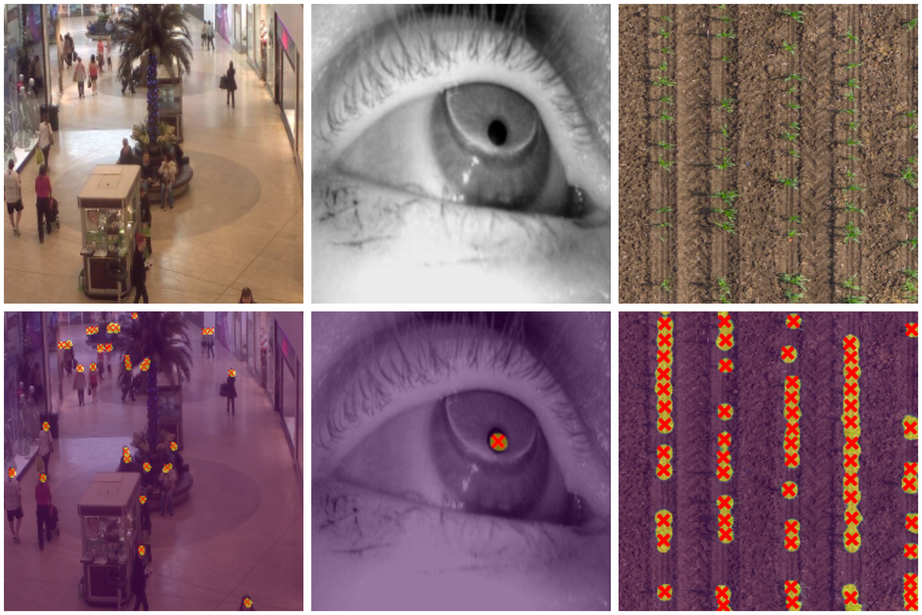
\includegraphics[width=0.5\textwidth]{fig/results/collage2x3.png}
\end{center}
    \caption{人的头部、瞳孔、植物中心的目标定位。(下面一排)
          热度图和交叉估计}
\label{fig:collage}
\end{figure}


在本文中,我们提出了一种修正的平均hausdorff距离作为CNN的损失函数来预测目标的位置。
我们的方法不要求在训练阶段使用边界框,并且在设计网络结构的时候也不需要知道目标的最大数量。
简单起见,我们只用一类目标来描述我们的方法,尽管这方法可以简单地扩展到多类目标。
我们的方法是目标不可知的,因此本文的讨论不包括任何关于目标特性的信息。
我们的方法将输入图像映射到一组坐标,并用不同的对象对其进行验证。
我们用三个数据集来验证我们的方法。
第一个数据集包含了从购物中心监控摄像头获取的图像,我们在其中定位了人头。
第二个数据集包含了人眼睛的图片,我们在其中定位了瞳孔的中心。
第三个数据集包含了由无人机航拍得到的谷物地的图像,我们定位了高度封闭(highly occluded)植物中心。


我们通过关键点检测实现目标定位的方法并不能取代边界框检测,尤其是对那些天生需要边界框的任务,比如自动裁剪。
此外,这种方法的一个局限性是,边界框标签包含了某种意义上的尺度,而关键点没有。

我们工作的贡献是:
\begin{itemize}
    \item 我们提出了一个用于目标定位的损失函数,我们称之为\textit{加权hausdoeff距离}(WHD),
          它克服了像素级的损失函数,如L2和hausdorff距离,的局限性。。
    \item 我们发展了一种用于估计图像中物体的位置和数量的方法,并且这种方法不使用任何边界框或者候选局域。
    \item 我们把目标定位问题表述为点之间最小距离的问题,与预测中使用的模型无关。
          这允许使用任何全卷积的网络架构设计。
    \item 我们的性能优于目前最先进的通用目标检测器,并且在不需要任何领域特定知识、数据增强或迁移学习的情况下,
            在人群计数场景下获得了不错的结果。
\end{itemize}

\section{相关工作}
\textbf{通用目标检测器。}
深度学习~\cite{deeplearningbook,nature}的最新进展提高了定位任务(如目标或关键点检测)的准确性。
对于通用的目标检测器,我们指的的是可以经过训练来检测任何一种或多种目标类型的方法,
例如Faster-RCNN~\cite{fastrcnn},SSD~\cite{ssd}或者YOLO~\cite{redmon2016you}。
在Fast R-CNN中,候选区域或者建议区域是通过诸如选择性搜索~\cite{selectivesearch}之类的经典方法生成的。
虽然网络的激活在不同的候选区域是共享的,但是系统不能端到端地进行训练。
目标检测器中的区域建议网络(RPNs)例如Faster R-CNN~\cite{fastrcnn,fasterrcnn}允许端到端的模型训练。
Mask R-CNN~\cite{maskrcnn}通过增添一个用于预测物体掩码的分支来扩展Faster R-CNN,
但是它和已经存在的用于边界框识别的分支并行。
Mask r-cnn可以通过生成一个单独的类来表示关键点的存在来估计人体姿态关键点。
Mask R-CNN中使用的损失函数是逐点的,使得关键点检测对分割掩模的对齐高度敏感。
SDD提供固定大小的边界框和分数,指示框中是否存在目标。
刚刚描述的方法要么在训练CNN时需要边界框要么要求知道图像中的最大目标数量。
在~\cite{huang2017}中,观察到一些诸如Faster R-CNN或者SSD的通用目标检测器在检测小物体时表现很差。



\textbf{计数和定位目标。}
计算一个图片中目标的数目并不是一件简单的任务。
在~\cite{lempitsky_2010}中,Lempitsky等人估计一个密度函数,它的积分相当于目标的数量。
在~\cite{shao_2015},Shao等人提出了两种定位目标物体的方法。
一种方法是首先计数然后定位,另一种方法是首先定位然后计数。

定位和计数人群的数量在很多应用中都是必要的,例如监控系统中的人群监控,新业务的调查,以及应急事件管理 \cite{lempitsky_2010,xiong2017}.
文献对此有多种研究,人群在时评中被检测和跟踪。
这些检测方法通常使用包围的人边界框作为基础。
在很多人互相重叠的情况下,获取一个人群中每一个人边界框是劳动密集且不准确的工作,比如运动会或者高峰时段的交通车站。
很多现代的方法通过估计一个密度图然后对其进行积分得到总人数来避免对边界框的需要。
在使用密度图的方法中,密度图的标签由人脑袋的标签构建。
这通常是通过将高斯核集中在每个头部的位置来完成的。
张等人~\cite{zhang2016}用多栏CNN估计密度图像,这个CNN可以在不同的尺度上学习特征。
在\cite{sam2017}中,Sam等人使用多个独立的CNN来预测不同人群密度下的密度图。
另外一个CNN对人群场景的密度进行分类,并将输入图像转发给相应的CNN。
黄等人~\cite{huang2018}建议将有关身体部位结构的信息合并到传统的密度图中,将人群计数重新定义为一个多任务问题。
其它的工作比如张等人~\cite{zhang2015}使用额外的信息比如被视为基本真理的映射图。

瞳孔跟踪和精确农业的方法通常是特定领域的。
在瞳孔跟踪中,必须在实际光照条件下对瞳孔中心进行解析。
广泛的应用中,从商业应用比如视频游戏~\cite{eyetracking_book},驾驶~\cite{applegan,copilot}或者微手术~\cite{fuhl2016_2}都依赖于瞳孔追踪。
在远程精准农业中,定位农田中的植物中心是至关重要的。
农学家用这些植物特性比如植物间距来预测未来的农田产量~\cite{thornley_1983,sui_2011,tokatlidis_2004,farnham2001,chauhan2011},而植物学家则利用这些特性来培育新的植物品种~\cite{araus_2014,neilson_2015}。
在~\cite{aich2018}中,Aich等人通过首先将植物分割成若干区域然后计数每个区域的植物数量来计算小麦的数量。

\textbf{豪斯多夫(Hausdorff)距离。}
豪斯多夫距离可以用来衡量两个点集之间的距离~\cite{attouch1991}。
豪斯多夫距离的改进版~\cite{dubuisson1994}被用到了很多任务之中,包括字符识别,~\cite{lu2001},人脸识别~\cite{lin2003}以及场景匹配~\cite{lin2003}。
Schutze等人~\cite{schutze2012}使用平均的豪斯多夫距离来衡量多目标优化的解决方案。
在~\cite{elkhiyari2017}中,Elkhiyari等人比较CNN根据多个豪斯多夫距离的变体提取的特征,以完成人脸识别任务。
在~\cite{fan2017}中,Fan等人使用Chamfer和Mover's距离以及一个新的神经网络结构,通过估计一些固定点的位置来进行三维重建。
豪斯多夫距离也是评价医学影像界分割边界质量的一个常用指标。

\section{平均豪斯多夫(Hausdorff)距离}
我们的工作是建立在豪斯多夫距离基础上的,我们将在本节中简洁地回顾它。
考虑两个非空的无序点集 $X$ 和 $Y$ 以及一个距离度量 $d(x,y)$,其中 $x \in X$ 并且 $y \in Y$。
函数 $d(\cdot,\cdot)$可以是任何度量标准。
在我们的例子中,我们使用欧几里得距离。
点集 $X$ 和 $Y$ 可能拥有不同数量的点。
让 $\Omega \subset \mathbb{R}^2$表示这个空间所有的点。
一般来说,$X \subset \Omega$ 和 $Y \subset \Omega$之间的距离被定义为
\begin{equation}
  \label{eq:hausdorff}
  d_{\text{H}}(X, Y) = \max \left\{ \sup_{x\in X} \inf_{y\in Y} d(x, y), \sup_{y\in Y} \inf_{x\in X} d(x, y) \right\}  .
\end{equation}

当考虑一个离散的有界的 $\Omega $,比如一张图片中的所有像素点,最小上界和最大下界都是可实现的,并且分别成为最大值和最小值。
这将豪斯多夫距离限制为
\begin{equation}
  \label{eq:dmax}
  d(X, Y) \le d_{max} = \max_{x\in \Omega, y \in \Omega} d(x, y)  ,
\end{equation}
当使用欧式距离时它相当于一张图像的对角线。
如果~\cite{attouch1991}所展示的,豪斯多夫距离是一个衡量标准。
因此,对于$\forall X, Y, Z \subset \Omega$,我们有以下的性质:
\begin{subequations}
\label{all1}
 \begin{align}
  \label{eq:hausdorff1}
     d_H(X, Y) & \ge 0 \quad   \\
  \label{eq:hausdorff2}
  d_H(X, Y) &= 0 \iff X = Y  \\
  \label{eq:hausdorff3}
  d_H(X, Y) &= d_H(Y, X)  \\
  \label{eq:hausdorff4}
  d_H(X, Y) &\le d_H(X, Z) + d_H(Z, Y)
 \end{align}
\end{subequations}

方程~\eqref{eq:hausdorff2}由$X$和$Y$是有界的导出,因为在我们的任务中像素的坐标空间 $\Omega $是离散的。
当要设计一个函数去衡量$X$和$Y$是多么相似的时候,这些特性是非常有用的。

\begin{figure}[t]
  \centering
  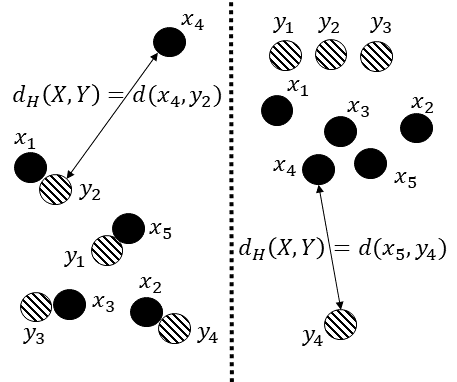
\includegraphics[width=0.3\textwidth]{fig/points.png}%

  \caption{点集$X=\{x_1, ..., x_5\}$(实心点)和$Y=\{y_1, ..., y_4\}$(虚线点)两种不同的布局的展示。
          尽管这两个点集之间有着明显的区别,但它们之间的豪斯多夫距离却因为最糟糕的离群点是一样的而相等。}
  \label{fig:points}
\end{figure}

豪斯多夫函数的一个缺点是它对离群点的高度敏感性~\cite{schutze2012,taha2015}。
图~\ref{fig:points}展示一个关于两个都有一个离群点的点集的例子。
为了避免这种情况,平均豪斯多夫距离被广泛地使用:
\begin{equation}
  \label{eq:AH}
  d_{\text{AH}}(X, Y) = \frac{1}{|X|} \sum_{x\in X} \min_{y\in Y} d(x, y) + \frac{1}{|Y|} \sum_{y\in Y} \min_{x\in X} d(x, y) ,
\end{equation}
其中$|X|$和$|Y|$分别是$X$和$Y$中点的数量。 

注意性质~\eqref{eq:hausdorff1},~\eqref{eq:hausdorff2}和~\eqref{eq:hausdorff3}仍然是真的,但是~\eqref{eq:hausdorff4}不再成立。
同时,平均豪斯多夫距离关于任何在$X$或者$Y$中的点是可微分的。

让$Y$包含正确的像素坐标,$X$是我们的估计。
理想情况下,我们将在训练卷积神经网络(CNN)时使用$d_{\text{AH}}(X, Y)$作为我们的损失函数。
当把平均豪斯多夫距离作为损失函数时我们发现两个限制。
首先,具有线性层的CNN隐式地决定了要估计$|X|$中点的数目,即最后一层的神经元个数。
这是一个缺陷,因为真正点的数目由图像自己的内容决定。
第二,全卷积网络(FCNs)比如U-Net~\cite{unet}可以指示在输出层中存在具有更高激活度的对象中心,但它们不返回像素坐标。
为了在学习过程中使用反向传播,损失函数对网络的输出必须是可微的。

\section{带权重的豪斯多夫(Hausdorff)距离}
\label{sec:whd}
为了克服这两种限制,我们对平均豪斯多夫距离的改进如下所示:

\begin{equation}
  \label{eq:WH}
    \begin{split}
        d_{\text{WH}}(p, Y) = &\frac{1}{\mathcal{S}+ \epsilon} \sum_{x\in \Omega} p_x \min_{y\in Y} d(x, y) + \\
        & \frac{1}{|Y|} \sum_{y\in Y} \underset{x\in \Omega}{M_\alpha} \left[\> p_x d(x, y) + (1 - p_x) d_{max} \, \right],
    \end{split}
\end{equation}
其中
\begin{equation}
  \label{eq:denom}
    \mathcal{S} = \sum_{x\in \Omega} p_x ,
\end{equation}

\begin{equation}
  \label{eq:genmean}
      \underset{a\in A}{M_\alpha} \left[ f(a) \right] = \left( \frac{1}{|A|} \sum_{a\in A} f^\alpha(a) \right) ^\frac{1}{\alpha} ,
\end{equation}

是由平均值产生,$\epsilon$被设定为$10^{-6}$。
我们称$d_{\text{WH}}(p, Y)$为加权豪斯多夫距离(WHD)。
$p_x \in [0, 1]$是网络在坐标点$x$处输出的一个单值。
最后一层网络的激活值可以使用sigmoid非线性激活函数将其限制在0和1之间。
注意$p$不需要标准化,即$\sum_{x\in \Omega} p_x = 1$是不必要的。
注意广义上讲,平均$M_\alpha \left[ \cdot \right]$对应于当$\alpha=-\infty$时的最小函数。
我们证明将改进应用于~\eqref{eq:AH}可以得到~\eqref{eq:WH}:
\begin{enumerate}
  \item 第一个项分母中的$\epsilon$在$p_x \approx 0 ~ \forall x \in \Omega$时提供了数值的稳定性。
  \item 当$p_x = \{0, 1\}$, $\alpha=-\infty$,并且$\epsilon = 0$时,加权的豪斯多夫距离变成了平均的豪斯多夫距离。
        我们可以将其解释为网络可以指示出完全确定的物体坐标。
        当$d_{\text{WH}}(p, Y) \geq 0$时,如果$x\in Y$,则全局最小值($d_{\text{WH}}(p, Y) = 0$)对应于$p_x = 1$,否则对应于0。
  \item 在第一项中,我们乘以$p_x$ 来惩罚在图像中附近没有真正点$y$的高激活值。
        换句话说,这个损失函数惩罚了不应该出现在这地方的估计点。
  \item 
        在第二项中,通过使用表达式\\ $f(\cdot) \vcentcolon = p_x d(x, y) + (1 - p_x) d_{max}$,我们迫使
      \begin{enumerate}
          \item
                如果$p_{x_0} \approx 1$,则$f(\cdot) \approx d(x_0, y)$。这意味着点$x_0$对损失的贡献和其在AHD(Equation~\eqref{eq:AH})中的贡献相同。
          \item 如果$p_{x_0} \approx 0$,$x_0 \neq y$,则$f(\cdot) \approx d_{max}$。
                然后,如果$\alpha = -\infty$,这个点$x_0$将不会对损失值产生贡献,因为这个“最小值”$M_{x\in \Omega}[\thinspace\cdot\thinspace]$会忽视$x_0$。
                如果存在一个其它点$x_1$和$y$更近且 $p_{x_1} > 0$,$x_1$将被“选择”,而不是$M[\thinspace\cdot\thinspace]$。
                否则,$M_{x\in \Omega}[\thinspace\cdot\thinspace]$的值将会很高。
                这意味着真实目标点周围的低激活值将被惩罚。
      \end{enumerate}
      注意$f(\cdot)$并不是唯一实施这两个约束($f|_{p_x = 1} = d(x, y)$ and $f|_{p_x = 0} = d_{max}$)的表达式。
      我们选择一个线性的函数,原因是它们的简单性和数值稳定性。
\end{enumerate}

WHD中的两项都是必要的。
如果第一项被移除,则这个平凡解是$p_x = 1 \quad \forall x \in \Omega$。
如果第二项被移除,则这个平凡解是$p_x = 0 \quad \forall x \in \Omega$。
这两种情况对$\alpha$取任何值都适用,其证明在附录中。
理想情况下,这个参数$\alpha \to -\infty$,因此$M_\alpha(\cdot) = ||\cdot||_{-\infty}$变成了取最小的操作符\cite{minimum}。
然而,这将使第二项与网络的输出持平。
对于一个给定的$y$,如果有另一个点$x_1$有更高的激活值且更靠近$y$,点$x_0$中$p_{x_0}$中的变化即远离$y$的点将被$M_{-\infty}(\cdot)$忽视。
在实践中,这是训练变得困难因为这个最小值对于输入来说并不是一个平滑的函数。
因此,我们用广义的平均$M_\alpha(\cdot)$来近似最小值,且$\alpha<0$。
$\alpha$越负,AHD和WHD越相似,以变的不那么光滑为代价。
在我们的实验中,$\alpha=-1$。
在第一项中没必要使用$M_\alpha(\cdot)$
因为$p_x$并不在最小值中,因此这一项已经对$p$可微。

如果在将图像喂给网络之前需要对其进行改变,我们可以规范化WHD来应对这种失真。
将原始图像记为$(S_o^{(1)}, S_o^{(2)})$同时将改变过后的图像记为$(S_r^{(1)}, S_r^{(2)})$。
In Equation~\eqref{eq:WH}, we compute distances in the original pixel space by replacing $d(x, y)$ with $d(\textbf{S} x, \textbf{S} y)$, where $x, y \in \Omega$ and 
在方程~\eqref{eq:WH},我们用$d(\textbf{S} x, \textbf{S} y)$来替代$d(x, y)$来在原始的像素空间中计算距离,其中$x, y \in \Omega$,并且
\begin{equation}
  \label{eq:normaliz}
    \textbf{S} = 
        \begin{pmatrix}
            S_o^{(1)} / S_r^{(1)}   &     0     \\
            0                             &     S_o^{(2)} / S_r^{(2)}  \\
        \end{pmatrix} .
\end{equation}


\subsection{相对于像素级损失函数的优势}
一种幼稚的替代方法是使用单热编码的图作为标签,定义$x \in Y$时$l_x = 1$,否则$l_x = 0$,
然后使用像素级的损失函数,比如均方误差(MSE)或者$L^2$标准,
其中$L^2(l, p) = \sum_{\forall x \in \Omega} |p_x - l_x|^2 \propto \text{MSE}(l, x)$。
像素级损失函数的问题是除非$x = y$,否则它们不能说明两个点$x\in \Omega$和$y\in Y$的距离有多斤。
换言之,对于绝大多数像素来说,它是平坦的,这使得训练变得不可行。
这个问题通过使用以$x\in Y$为中心高斯分布的均方误差在局部得到缓解\cite{tompson2015efficient}。
对比之下,方程~\eqref{eq:WH}中的WHD将会随着$x$靠近$y$而减小,使得损失函数可以全局最小值之外提供训练所需的信息。

%-------------------------------------------------------------------------
\section{CNN架构以及位置估计}
\label{sec:cnn}

\begin{figure}[t]
\begin{center}
   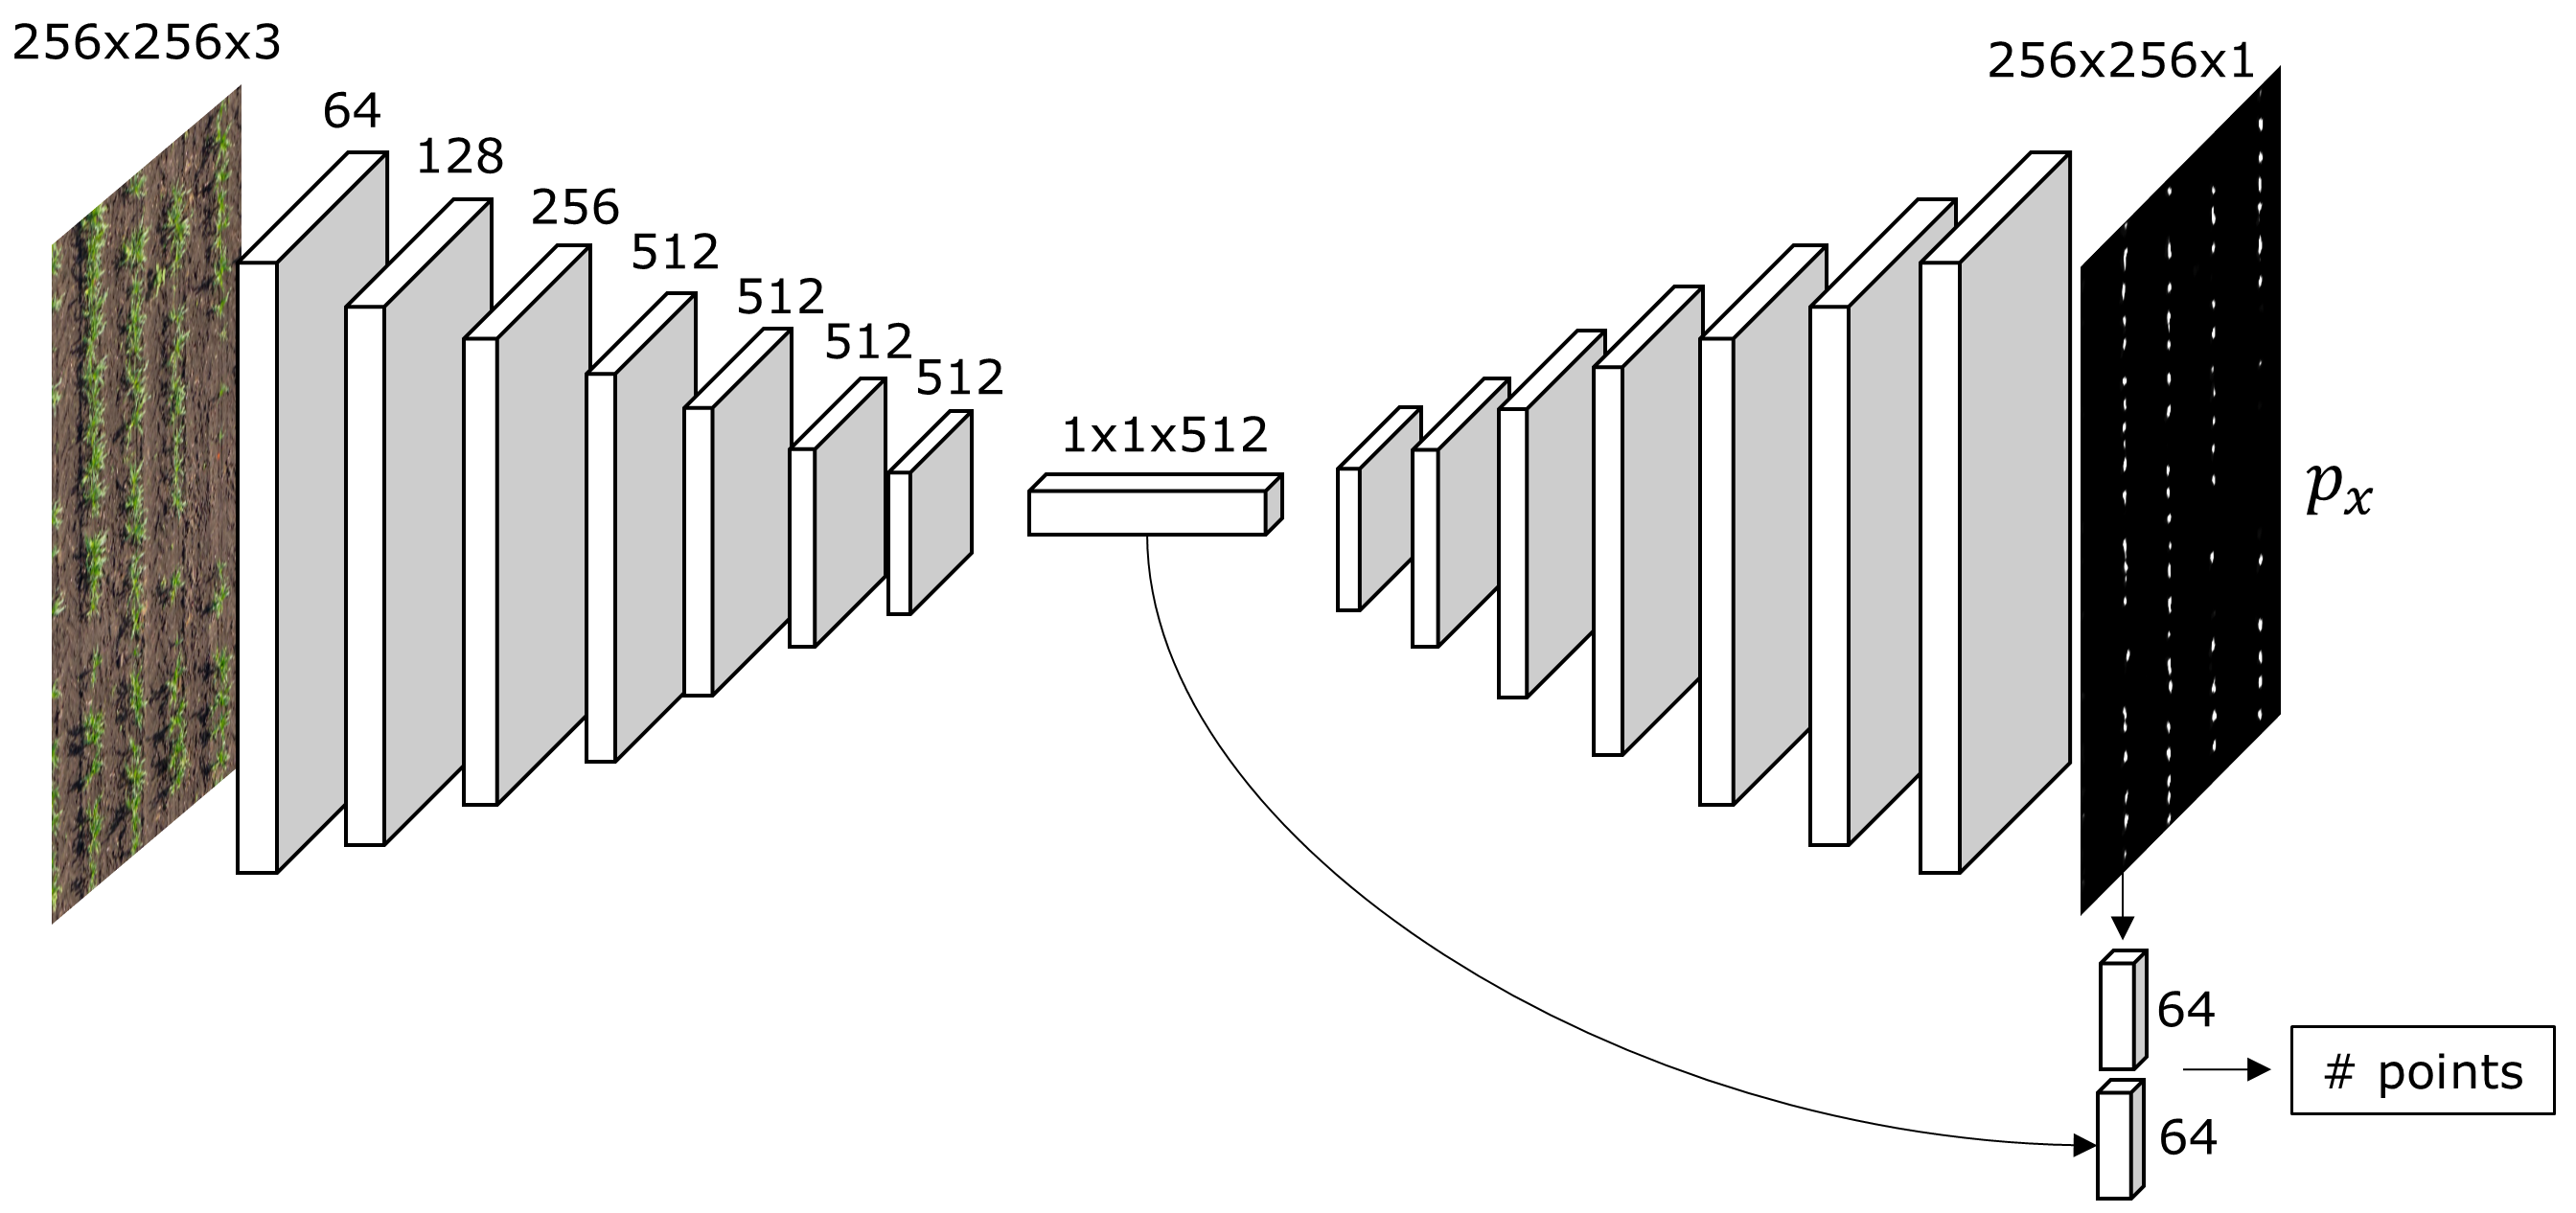
\includegraphics[width=0.5\textwidth]{fig/unetlike.png}
\end{center}
   \caption{
            用于目标定位的FCN架构,最小限度的改编自U-Net~\cite{unet}架构。
            我们添加了一个小的全连接层,它将最深层的特征和估计出的概率密度图结合起来去回归得到点的数量。
            }
\label{fig:unet_like}
\end{figure}
在这个部分,我们将描述我们使用的全卷积网络,以及我们我们怎么估计最终的位置。
我们想强调这个网络结构的设计在我们的工作中并不是一个有意义的贡献。
因此我们没有尝试去优化它。
我们的主要贡献是使用加权的豪斯多夫距离作为我们的损失函数。
我们采用了U-Net的网络结构\cite{unet}并对为了这个任务做了微小的修改。
类似于U-Net的网络已经被证明,在训练时采用条件对抗生成网络的设置或~\cite{pix2pix}者使用一个精心调试的损失函数的情况下,它有能力精准地将输入图片映射到输出图片上。
图~\ref{fig:unet_like}展示了U-Net的沙漏设计。
为了简单起见,没有显示出编码器中每一层与解码器中之对称的层之间的残差连接。

这个FCN有两个区别很大的块。
第一个块遵循了CNN典型的结构。
它由两个$3\times3$卷积(带1填充)重复应用组成,其中每一层紧跟了一个批量归一化和一个整流线性单元(ReLU)。
在ReLU之后,我们使用了不长为2的$2\times 2$的最大池化操作来进行降采样。
在下采样的步骤中,我么将特征的通道数加倍,开始为64通道,在最后5层使用512通道。
第二个块由以下元素重复应用组成:一个双线性上采样,与一个来自下采样的特征图拼接,以及两个$3 \times 3$的卷积,其中每一个跟随一个批量归一化和一个RELU激活层。
最后一层是一个将网络输出映射到一个单通道的的卷积层,$p$。

为了估计目标的图片中目标的数量,我们添加了一个将最深层的特征和估计的概率图结合起来的分支。
这个分支将两个特征(一个$1\times 1 \times 512$特征向量和$256 \times 256$概率图)结合到一个隐藏层中,然后使用一个128维的特征向量输出一个值。
然后我们使用看一个ReLU激活函数来保证输出时正的,同时将其舍入到最近的整数来获得我们最终对目标数量的估计,$\hat{C}$。

虽然我们使用了特定的网络结构,其它任何结构也可以被使用。
唯一的要求是网络的输出图像必须和输入图像的尺寸相同。
选择FCN源自于其输出作为WHD(方程~\eqref{eq:WH})中的权重($p_x$)的自然解释。
在之前的工作中\cite{elkhiyari2017,fan2017},平均豪斯多夫距离的变体已经被成功地应用在直接估计点集的非FCN网络中。
但是,在这些案例中,被估计集合的大小已经被最后一层的尺寸给确定了。
为了定位未知数量的物体,网络必须有能力来估计数量可变的物体位置。
因此,我们可以设想,只要网络的输出使用方程\eqref{eq:WH}中的$p$,WHD也可以应用到非FCN网络当中。

我们用于训练网络的的损失函数是一个方程\eqref{eq:WH}和一个用于对目标数量进行回归的平滑的$L_1$损失函数的组合。
最终的损失函数是
\begin{equation}
  \label{eq:loss}
\begin{split}
    \mathcal{L}(p, Y) = d_{WH}(p, Y) + \mathcal{L}_{\text{reg}}(C - \hat{C}(p)),
 \end{split}
\end{equation}

其中$Y$是包含了图像中目标的真正坐标的集合,$p$是网络的输出,$C = |Y|$,以及$\hat{C}(p)$是对目标数量的估计。
$\mathcal{L}_{\text{reg}}(\cdot)$是回归项,这一项我们使用平滑的$L_1$或者Huber损失\cite{huber1964},定义为
\begin{equation}
    \mathcal{L}_{\text{reg}}(x) =
    \begin{cases}
        0.5x^2,& \text{for} |x| < 1 \\
        |x| - 0.5,& \text{for} |x| \geq 1 \\
   \end{cases}
\end{equation}
当回归误差较大时,这种损失对离群点是鲁棒的,同时在原点是可微的。

\begin{figure}[t]
\begin{center}
   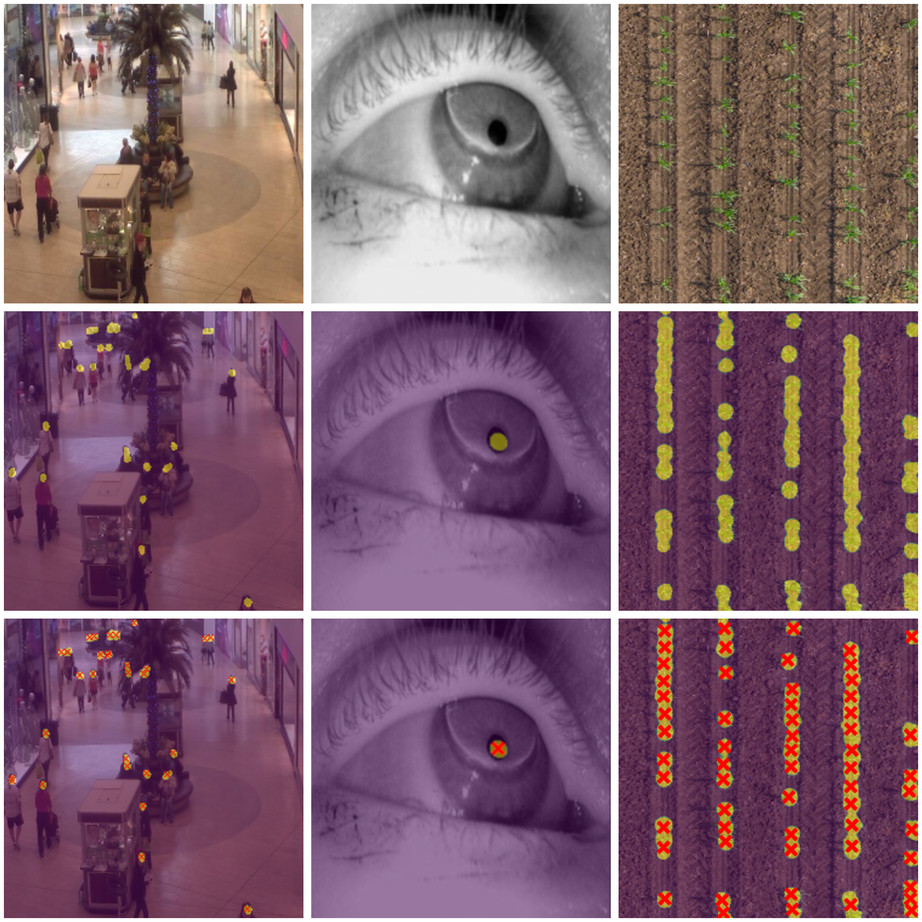
\includegraphics[width=0.5\textwidth]{fig/results/collage3x3.png}
\end{center}
   \caption{
            第一行,输入图像
            第二行:网络的输出(文本中的$p$)覆盖在输入图像上。
            这个可以被认为是一个目标定位的显著图。
            第三行:估计目标的位置使用了红色十字标记。}
\label{fig:collage_clusters}
\end{figure}


网络输出一个显著图$p$,用$p_x \in [0,1]$指示在像素点$x$有目标物体的置信度。
图\ref{fig:collage_clusters}在第二行展示了$p$。
在评估过程中,我们的最终目标是获得$\hat{Y}$,例如,对所有的目标位置的估计。
为了将$p$转化为$\hat{Y}$,我们对$p$进行了阈值来获得像素$T = \left\{ x\in \Omega ~ | ~ p_x > \tau \right\}$。
我们可以使用三种方法来决定使用哪一个$\tau$。
\begin{enumerate}
    \item 对于所有的图像使用一个常数$\tau$。
    \item 使用Otsu阈值\cite{otsu}来为每一幅图片寻找一个合适的$\tau$。
    \item 使用Beta混合模型的阈值(BMM)。
          该方法使用\cite{bmm}中描述的算法将两个Beta分布的混合拟合为$p$值,然后取平均值最高的分布的平均值作为$\tau$。
\end{enumerate}
图\ref{fig:collage_clusters}第三行展示了一个对显著图$p$阈值化后得到的结果的例子。
然后,我们将高斯混合模型拟合都$T$点。
这是使用期望最大化(EM)\cite{em}算法和估计的植物数量$\hat{C}$来完成的。

拟合的高斯平均数被认为最终的估计值$\hat{Y}$。
图\ref{fig:collage_clusters}的第三行展示标记了红色十字的最终估计物体。
需要注意的是,即使FCN结果良好,即每个目标的位置都一个集群,如果$|\hat{C} - C | > 0.5$,EM也有可能不能产生正确的目标位置。
在图\ref{fig:collage_clusters}的第一列可以看到一个例子,一个人头被错误地估计为两个人头。

%-------------------------------------------------------------------------
\section{实验结果}
我们用三个数据集来评价我们地方法。
第一个数据集包含来自一个商场监控摄像头拍摄的2000张照片。
它包含已经标注的人群中人头的位置。
这个数据集是可以在\url{http://personal.ie.cuhk.edu.hk/~ccloy/downloads\_mall\_dataset.html} \cite{loy2013}公开访问的。
80\%, 10\% and 10\% 的随机打乱的图片分别被作为训练集验证集和测试集。

第二个数据集在\cite{fuhl2015}中以罗马字母出现,并且在\url{http://www.ti.uni-tuebingen.de/Pupil-detection.1827.0.html}公开提供。
它包含2135张单只眼睛的图片,目标是检测瞳孔的中央。
它也是随意按照80/10/10 \%的比例被划分为训练集,验证集和测试集。

第三个数据集包含一个农田的航拍图像,这些图像是由一个无人机在40m的海拔拍摄的。
这些图像被拼接在一起,生成了一个$6,000 \times 12,000$的$0.75 $cm/每像素分辨率的正射图像,如图\ref{fig:ortho}所示。
图像中所有植物的中心都是真实的,共计15208个独一无二的植物中心。
这个马赛克图像被分割,左边百分之80用于训练,中间的百分之10用于验证,右边百分之10用于测试。
在每个区域内,随机生成图像作物。
这些随机作物的高度和宽度在100到600像素之间均匀分布。
我们在训练区域随机抽取50000张图片,验证区域和测试区域各随机抽取$5,000$张图片。
注意这些图片可能会高度重叠。
我们使第三个数据集可以在\url{https://engineering.purdue.edu/~sorghum/dataset-plant-centers-2016}被公开访问。
我们相信这个数据集对社区是有用的,因为由于植物的高度封闭性,这是一个极大的挑战。

\begin{figure}[t]
\begin{center}
   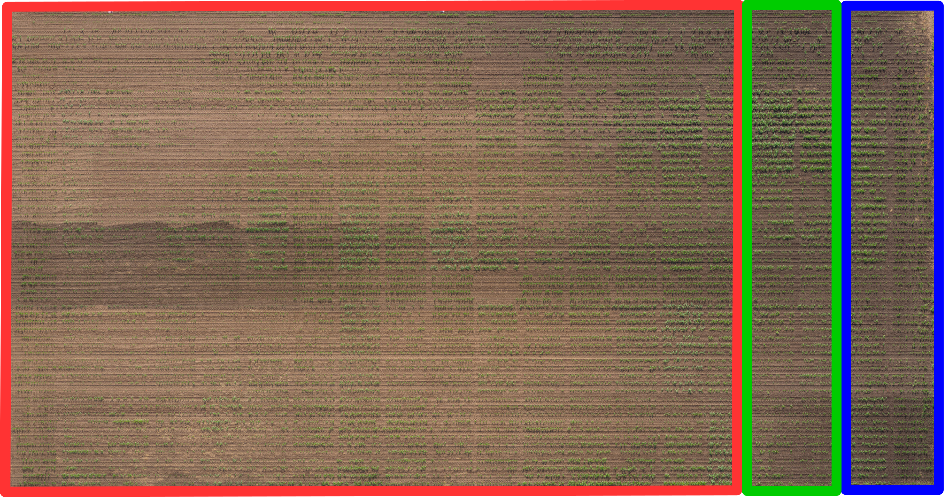
\includegraphics[width=0.7\linewidth]{fig/field/split.png}
\end{center}
   \caption{
            一个拥有15208张图片的拼接图像。红色区域用于训练,绿色区域用于验证,蓝色区域用于测试。}
\label{fig:ortho}
\end{figure}

所有的图片都被调整为$256 \times 256$,因为这是我们网络结构允许的最小大小。
真实目标的位置也被相应的缩放。
对于数据增强,我们使用了随机水平翻转。
对于植物的数据集,我们也使用了竖直的翻转。
我们设置方程~\eqref{eq:genmean}中的$\alpha=-1$。
我们也实验了$\alpha=-2$,但没有明显的提升,但是我们没有尝试去寻找一个最佳值。
我们为每个数据集重新训练网络,即我们不使用预先训练的权重。
对于商场和植物的数据集,我们设置批大小(batch size),使用Adam优化器~\cite{kingma_2014,amsgrad}以及将学习率设置为$10^{-4}$,动量设置为0.9。
对于眼瞳的数据集,我们通过移除5各个中间层来降低网络的大小,使用批大小(batch size)为64,随机梯度下降法的学习率为$10^{-3}$以及动量设置为0.9。
在每一轮训练的结束,我们在验证集上衡量方程\eqref{eq:AH}中的平均豪斯多夫距离(AHD),
同时选择在验证集上AHD最小的那一轮。

关于衡量标准,我们报告了准确率,召回率,F得分,AHD,平均绝对误差(MAE),根均方误差(RMSE)以及平均绝对百分比误差(MAPE)。
\begin{equation}
    \text{MAE} = \frac{1}{N}\sum_{i=1}^{N}| e_i |,  \quad \text{RMSE} = \sqrt{\frac{1}{N}\sum_{i=1}^{N} \big| e_i \big|^2}
  \label{eq:MAEandRMSE}
\end{equation}
\begin{equation}
    \text{MAPE} = 100 \frac{1}{N} \sum_{\substack{i=1 \\ C_i \neq 0}}^{N}\frac{\big| e_i \big|}{C_i}
  \label{eq:MAPE}
\end{equation}

其中$e_i = \hat{C_i} - C_i$,以及$N$是图片的数量,$C_i$是第$i$张图片中正确的目标个数,$\hat{C}_i$是我们估计的目标个数。

如果估计位置与真值点的距离不超过$r$,则计为真阳性。
如果估计位置在距离$r$处没有任何真值点,则计为假阳性。
如果一个真值点再距离$r$内没有估计点,则记为假阴性。
准确率是我们估计的点中,真阳性的比例。
召回率是真实位置中,我们检测出来的比率。
F分数是准确率和召回率的调和平均数。
注意,即使我们估计每个真值点附近有多个目标位置,也可以达到100\%的精度和召回率。
这将不是一个理想的定位。
将这个考虑在内,我们同时报告了可以指示出目标数量是否正确的度量标准(MAE,RMSE和MAPE)。
AHD可以被解释为以像素为单位的平均误差。

图~\ref{fig:precnrec}展示了F分数作为$r$的函数。
注意,$r$是只是一个的评价参数。
在训练和测试时并不需要它。
MAE,RMSE以及MAPE在表\ref{tab:results1}中展示了出来。
注意,除了在眼瞳的数据集中去掉中间层,我们对所有任务都使用了相同的结构。
并且,在瞳孔检测中,我们知道图片中只有一个目标。
因此,回归是不必要的,同时我们可以移除方程~\eqref{eq:loss}中的回归项以及固定$\hat{C_i} = C_i = 1 ~ \forall i$。

一种简单的目标定位方法是使用通用目标检测器,比如Faster R-CNN\cite{fasterrcnn}。
我们可以通过构造以每个标记点为中心的固定大小的边界框来训练这些检测器。
然后,每个边界框的中心可以被认为是估计的位置。
我们使用$20 \times 20$大小的包围盒(近似平均的头部和瞳孔大小)和 $16\times 16$和$32 \times 32$的锚大小。
请注意,这些参数可能是次优的,即使它们是为匹配对象类型而选择的。
我们用于SoftMax分数的阈值为0.5,用于联合交叉口的阈值为0.4,
因为他们将验证集上的AHD最小化。
我们使用VGG-16结构~\cite{vgg}并用学习率为$10^{-3}$,动量为0.9的随机梯度下降法对其进行训练。
对于瞳孔数据集,我们总选择得分最高的边界框。
我们实验观察到,Faste R-CNN难以检测到非常小的且相互非常近的目标。
表格~\ref{tab:mall}-\ref{tab:plants}展示了Faster R-CNN在商场,瞳孔以及植物数据集上的效果。
注意商场和植物数据集有很多很小且相互重合的目标,这是对Faster R-CNN最大的挑战。
这个行为和\cite{huang2017}中观察的一致,
其中,所有的通用目标检测器表现得很差,Faster R-CNN在最好的情况下只有5\%的平均正确率。

我们还使用均值漂移\cite{meanshift}代替高斯混合(GM)来检测局部极大值。
但是,均值漂移容易检测出多个局部最大值,而GM对离群点的鲁棒性更强。
在我们的实验中,我们观察到它的准确率和召回率要比使用GM差得多。
更重要得是,使用均值漂移使验证慢了一个数量级。
在使用scikit learn实现时,mean-shift算法在其中一幅图像上运行的平均时间是12秒,而使用期望最大化拟合gm大约需要0.5秒。

\begin{figure}[t]
\centering     %%% not \center
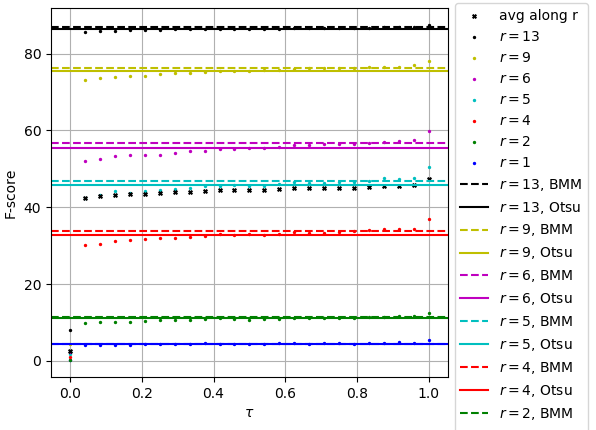
\includegraphics[width=0.85\linewidth]{fig/threshold/fscore_vs_tau.png}
    \caption{
            $\tau$阈值对F分数的影响。}
    \label{fig:tau}
\end{figure}

\begin{figure}[t]
\centering     %%% not \center
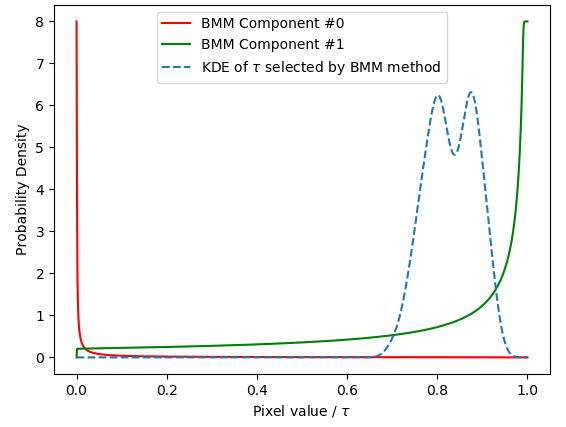
\includegraphics[width=0.85\linewidth]{fig/threshold/bmm_stats.png}
    \caption{
             Beta混合模型拟合$p_x$值,阈值$\tau$采用BMM方法。}
    \label{fig:bmm}
\end{figure}

我们还研究了参数$\tau$的影响,使用第~\ref{sec:cnn}节中的展示的三种方法。
有人可能会认为,这个参数可能是某些指标之间的一种折衷,并且应该进行交叉验证。
在实际应用中,我们发现$\tau$不平衡准确度和召回率,因此精确召回曲线没有意义。
相反,我们在图~\ref{fig:precnrec}画出了F值作为$r$的函数。
除此之外,交叉验证$\tan$意味着找到所有图像的“最佳”值。
图~ref{fig:tau}展示出使用适应性的阈值化方法效果更好(Otus或者BMM)。
注意BMM阈值化方法(虚线)总是比Otus(实线)和大多数固定的$\tau$效果好。
为了证明BMM方法的适当性,请注意,在图~\ref{fig:collage_clusters}中,估计图中的大多数值都非常高或非常低。
这使得Beta分布比正态分布(如otsu方法中使用的)更适合对$p_x$建模。
图~\ref{fig:bmm}显示了用BMM方法自适应选择的$\tau$值的拟合BMM和核密度估计。



\begin{table}[t]
  \centering
  \caption{
           使用$r=5$时,我们方法目标定位的结果。
           度量标准在方程~\eqref{eq:AH},~\eqref{eq:MAEandRMSE}-\eqref{eq:MAPE}中进行了定义。
           在瞳孔数据集中,因为总是只有一个瞳孔($\hat{C} = C = 1$),故没有展示回归的度量标准。
           图\ref{fig:precnrec}展示了其它值得F分数。}
  \begin{tabular}{lllll}
  \toprule
  \textbf{衡量标准} & \specialcellbold{商场 \\ 数据集} & \specialcellbold{瞳孔 \\ 数据集}  & \specialcellbold{植物 \\ 数据集} & \textbf{平均值}\\
  \midrule
  准确率 & 95.2\%  & 99.5\%  & 88.1\% & 94.4\%  \\
  召回率 & 96.2\%  & 99.5\% & 89.2\% & 95.0\%  \\
  F分数 & 95.7\%  & 99.5\% & 88.6\% & 94.6\%  \\
  AHD & 4.5 px & 2.5 px   & 7.1 px & 4.7 px \\
  MAE & 1.4 & -    & 1.9 & 1.7  \\
  RMSE & 1.8 & -     & 2.7 & 2.3  \\
  MAPE & 4.4\% & -    & 4.2\% & 4.3 \%  \\
  \bottomrule
  \end{tabular}
  \label{tab:results1}
  \end{table}

  \begin{table}
    \centering
    \caption{
            商场数据集得头部定位结果,使用$r=5$。}
    \begin{tabular}{lll}
    \toprule
    \textbf{衡量标准}  & \textbf{Faster-RCNN} &  \textbf{我们的} \\
    \midrule
    准确率 & 81.1\%  & \textbf{95.2 \%} \\
    召回率 & 76.7\%   & \textbf{96.2 \%} \\
    F分数 & 78.8 \%   & \textbf{95.7 \%} \\
    AHD & 7.6 px & \textbf{4.5 px} \\
    MAE & 4.7 & \textbf{1.4}  \\
    RMSE & 5.6 & \textbf{1.8} \\
    MAPE & 14.8\% & \textbf{4.4 \%} \\
    \bottomrule
    \end{tabular}
    \label{tab:mall}
    \end{table}
    
    \begin{table}\centering
    \caption{
             瞳孔检测结果,使用$r=5$。
             因为只有一个估计和一个真实目标,故准确率和召回率相同}
    \begin{tabular}{llll}
    \toprule
        \textbf{方法} & \textbf{准确率} & \textbf{召回率} &  \textbf{AHD} \\
        \midrule
        Swirski \cite{swirski2012} & 77 \% & 77 \%  & - \\
        ExCuSe \cite{fuhl2015} & 77 \% & 77 \%  & - \\
        Faster-RCNN & 99.5 \% & 99.5 \% &  2.7 px  \\
        \textbf{Ours} & \textbf{99.5} \% & \textbf{99.5} \% & \textbf{2.5 px}  \\
    \bottomrule
    \end{tabular}
    \label{tab:pupil}
    \end{table}
    
    \begin{table}
    \centering
    \caption{
            使用植物数据集进行植物定位的结果,使用$r=5$。}
    \begin{tabular}{lll}
    \toprule
    \textbf{衡量标准}  & \textbf{Faster-RCNN} &  \textbf{我们的} \\
    \midrule
    准确率 & 86.6 \%  & \textbf{88.1 \%} \\
    召回率 & 78.3 \%   & \textbf{89.2 \%} \\
    F分数 & 82.2 \%   & \textbf{88.6 \%} \\
    AHD & 9.0 px & \textbf{7.1 px} \\
    MAE & 9.4 & \textbf{1.9}  \\
    RMSE & 13.4 & \textbf{2.7} \\
    MAPE & 17.7 \% & \textbf{4.2 \%} \\
    \bottomrule
    \end{tabular}
    \label{tab:plants}
    \end{table}

    \begin{figure}[htbp]
      \subfigure{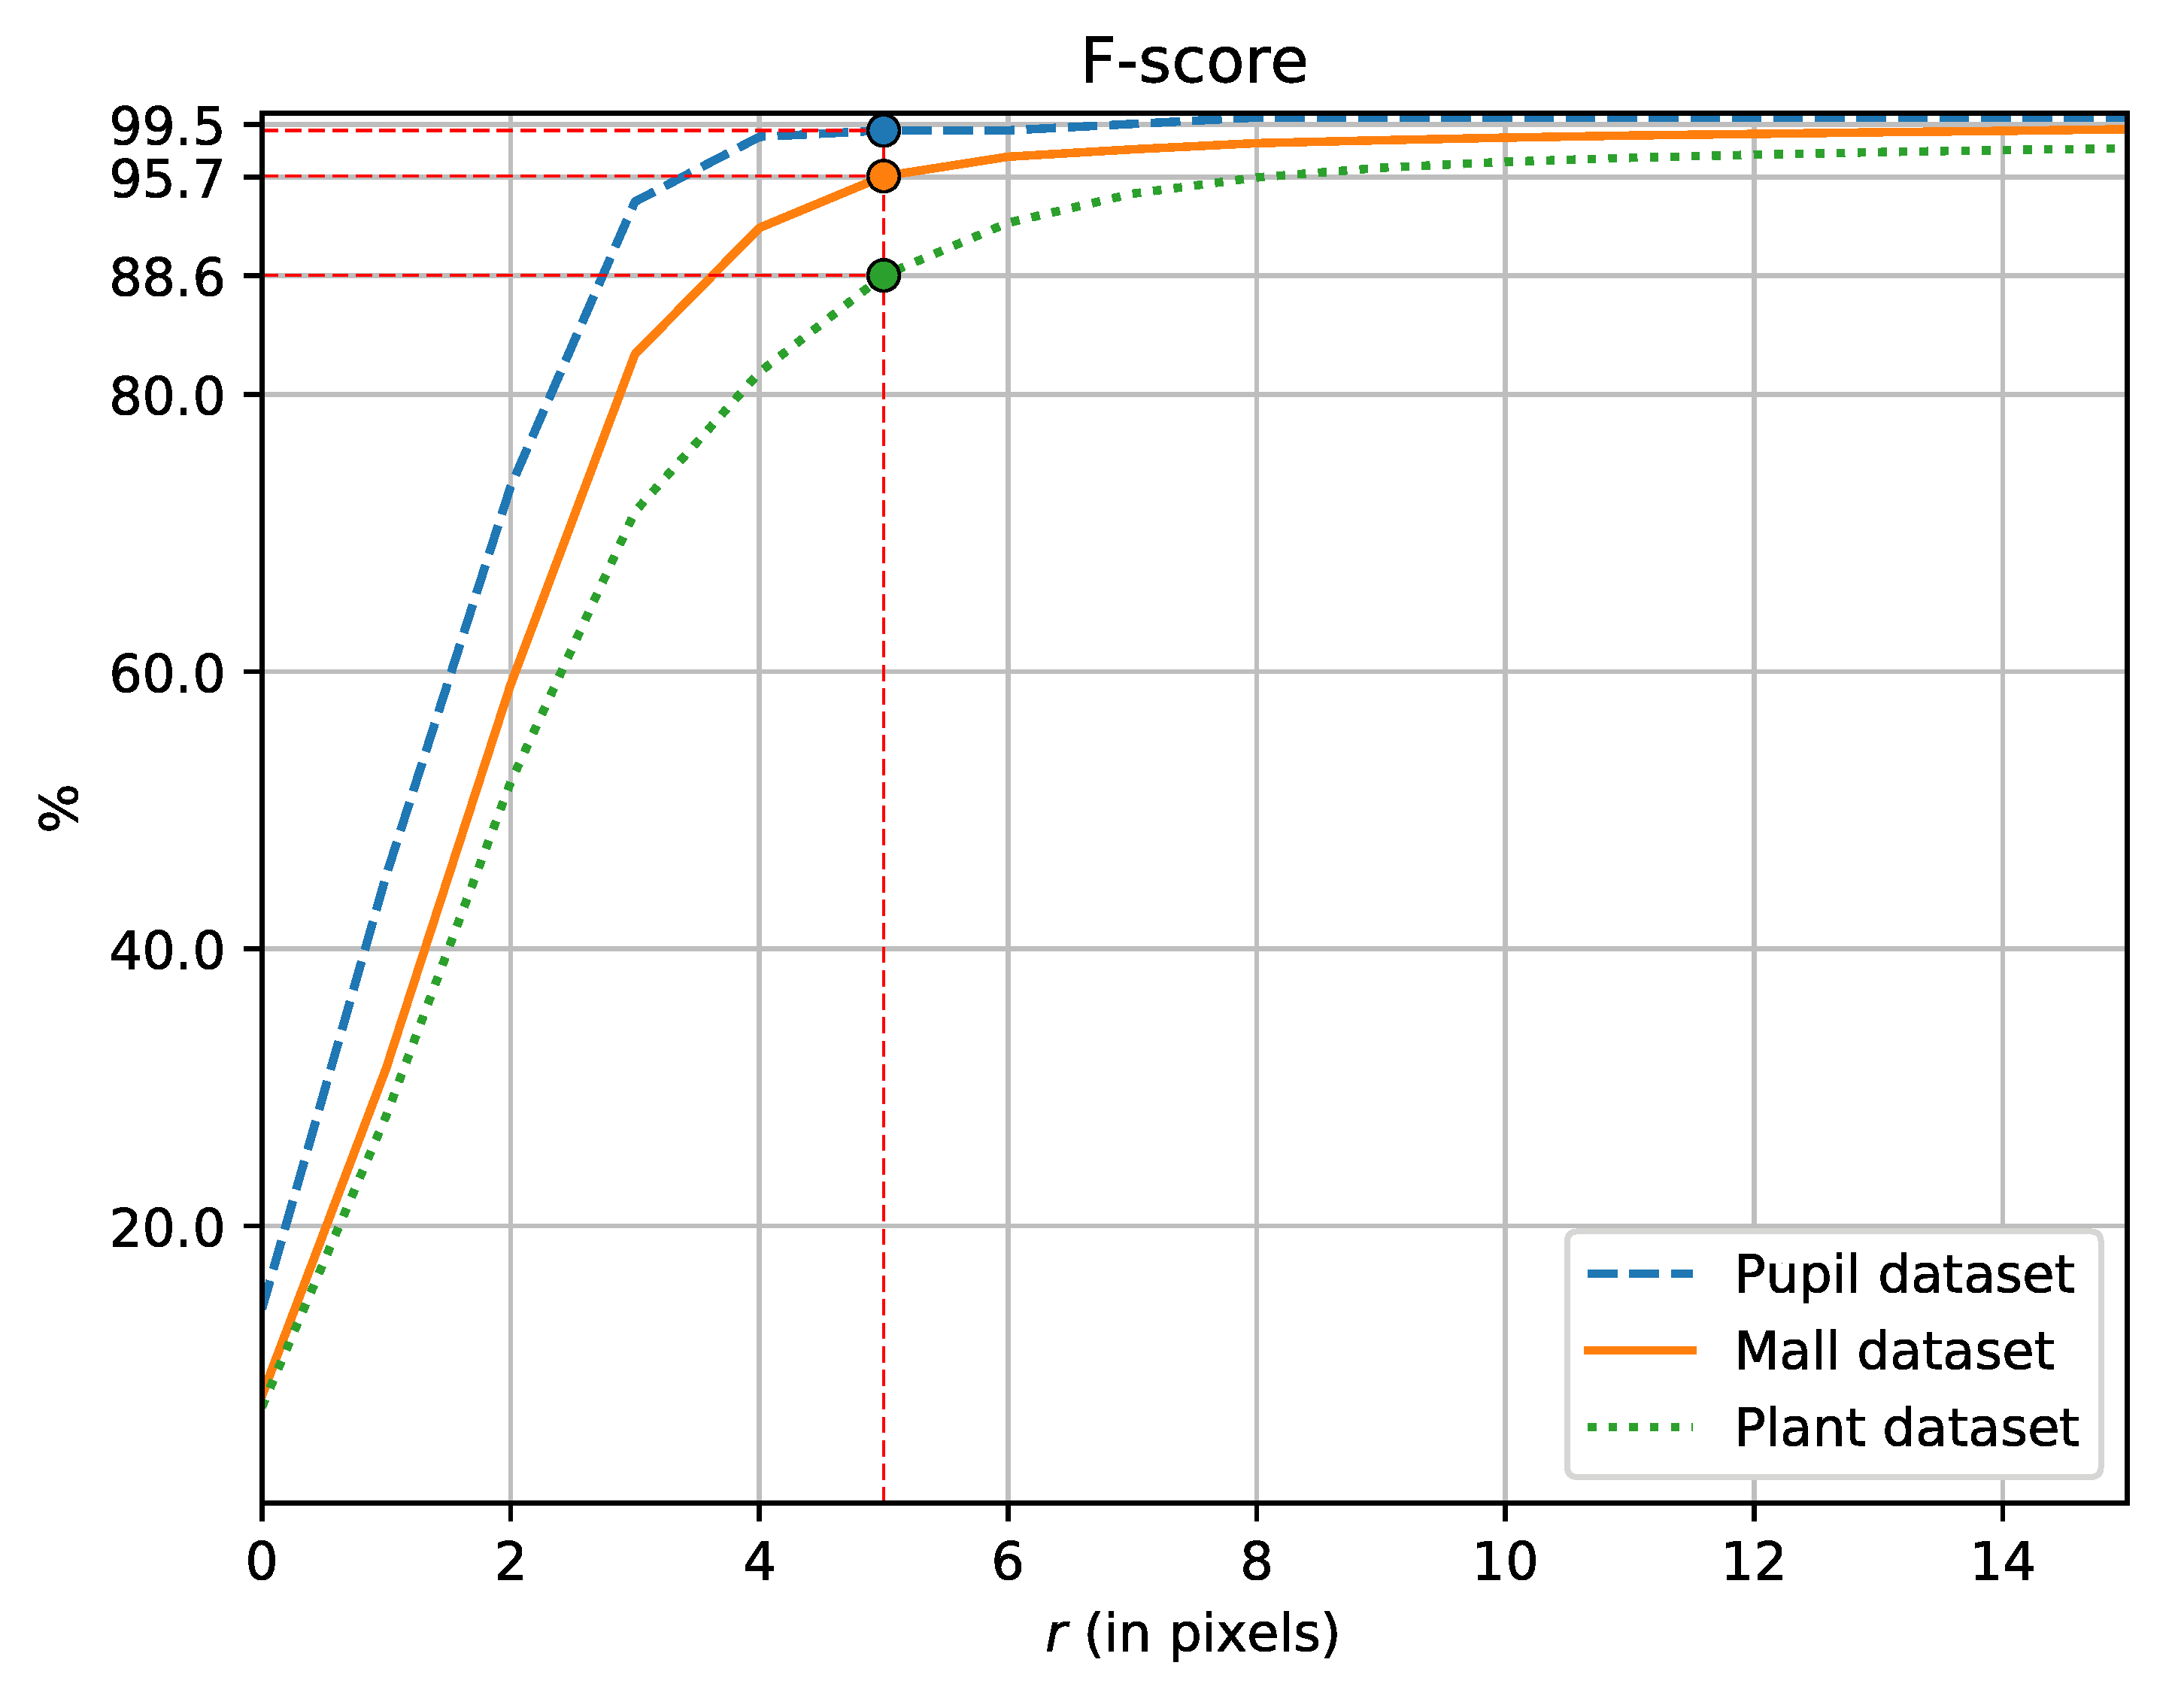
\includegraphics[width=0.9\linewidth]{fig/precnrec/f-score.png}}
      \caption{
               F分数作为$r$的函数,
               正确与估计的目标位置之间的最大距离,以判断其正确与否。
               一个较高的$r$使正确地地位更加简单。}
      \label{fig:precnrec}
    \end{figure}

最后,因为我们的方法同时定位和计数目标,所以它可以被用为一个计数技术。
我们还使用\cite{zhang2016}中提供的上海理工大学B部分数据集对我们的人群计数技术进行了评估,
并获得了19.9的MAE。
尽管我们没有超过专门针对人群计数进行微调的最新方法\cite{li2018},
但我们可以使用我们的通用方法获得可比的结果。
我们期望将来的改进,比如架构的改变或者使用迁移学习来进一步提高性能。


使用PyTorch实现的使用加权豪斯多夫距离作为损失函数的代码和训练的模型可以在\url{https://github.com/javiribera/locating-objects-without-bboxes}上获得。






\section{结论}
我们提出了一个损失函数,用于在不需要包围盒边界框的图像中的目标定位。
这个损失函数时平均豪斯多夫距离(AHD)的改进,用来衡量来两个无序点集之间的距离。
为了使AHD相对于网络输出可微,我们在估计目标位置时考虑了网络的确定性。
网络的输出是一个用来定位的显著性图和一个估计目标的数量的数字。
我们的方法不受目标最大数量的限制,不需要边界框,不需要候选区域或者滑动窗。
这个方法可以应用在边界框难以获得或者目标尺寸太小以至于边界框的标定不实际的任务。
我们在三个数据集上衡量了我们的数据集,并且效果优于通用目标检测器和特定任务技术。
未来的工作将包括在开发出在单一网络中的多目标定位器,
以及使用更多现代的CNN架构。

\vspace{1em}

{
\small \textbf{致谢:}
    这项工作由高级研究项目局能源部(ARPA-E)资助。
    美国能源部,授权编号DE-AR0000593。
    本文作者的观点和意见并不一定反映美国政府或其任何机构的观点和意见。
    因为本文中使用的正射图像,我们感谢Ayman Habib教授。
    联系信息:Edward J. Delp, \texttt{\href{mailto:ace@ecn.purdue.edu}{ace@ecn.purdue.edu}}
}

\clearpage

\bibliographystyle{ieee}
\bibliography{ref}

\renewcommand{\thesection}{\Alph{section}}

\end{document}
